\documentclass[tikz, border=2mm]{standalone}
\usepackage{tikz}
\usetikzlibrary{
    positioning,
    fit,
    arrows.meta,
    calc,
    shapes.geometric
}

\begin{document}

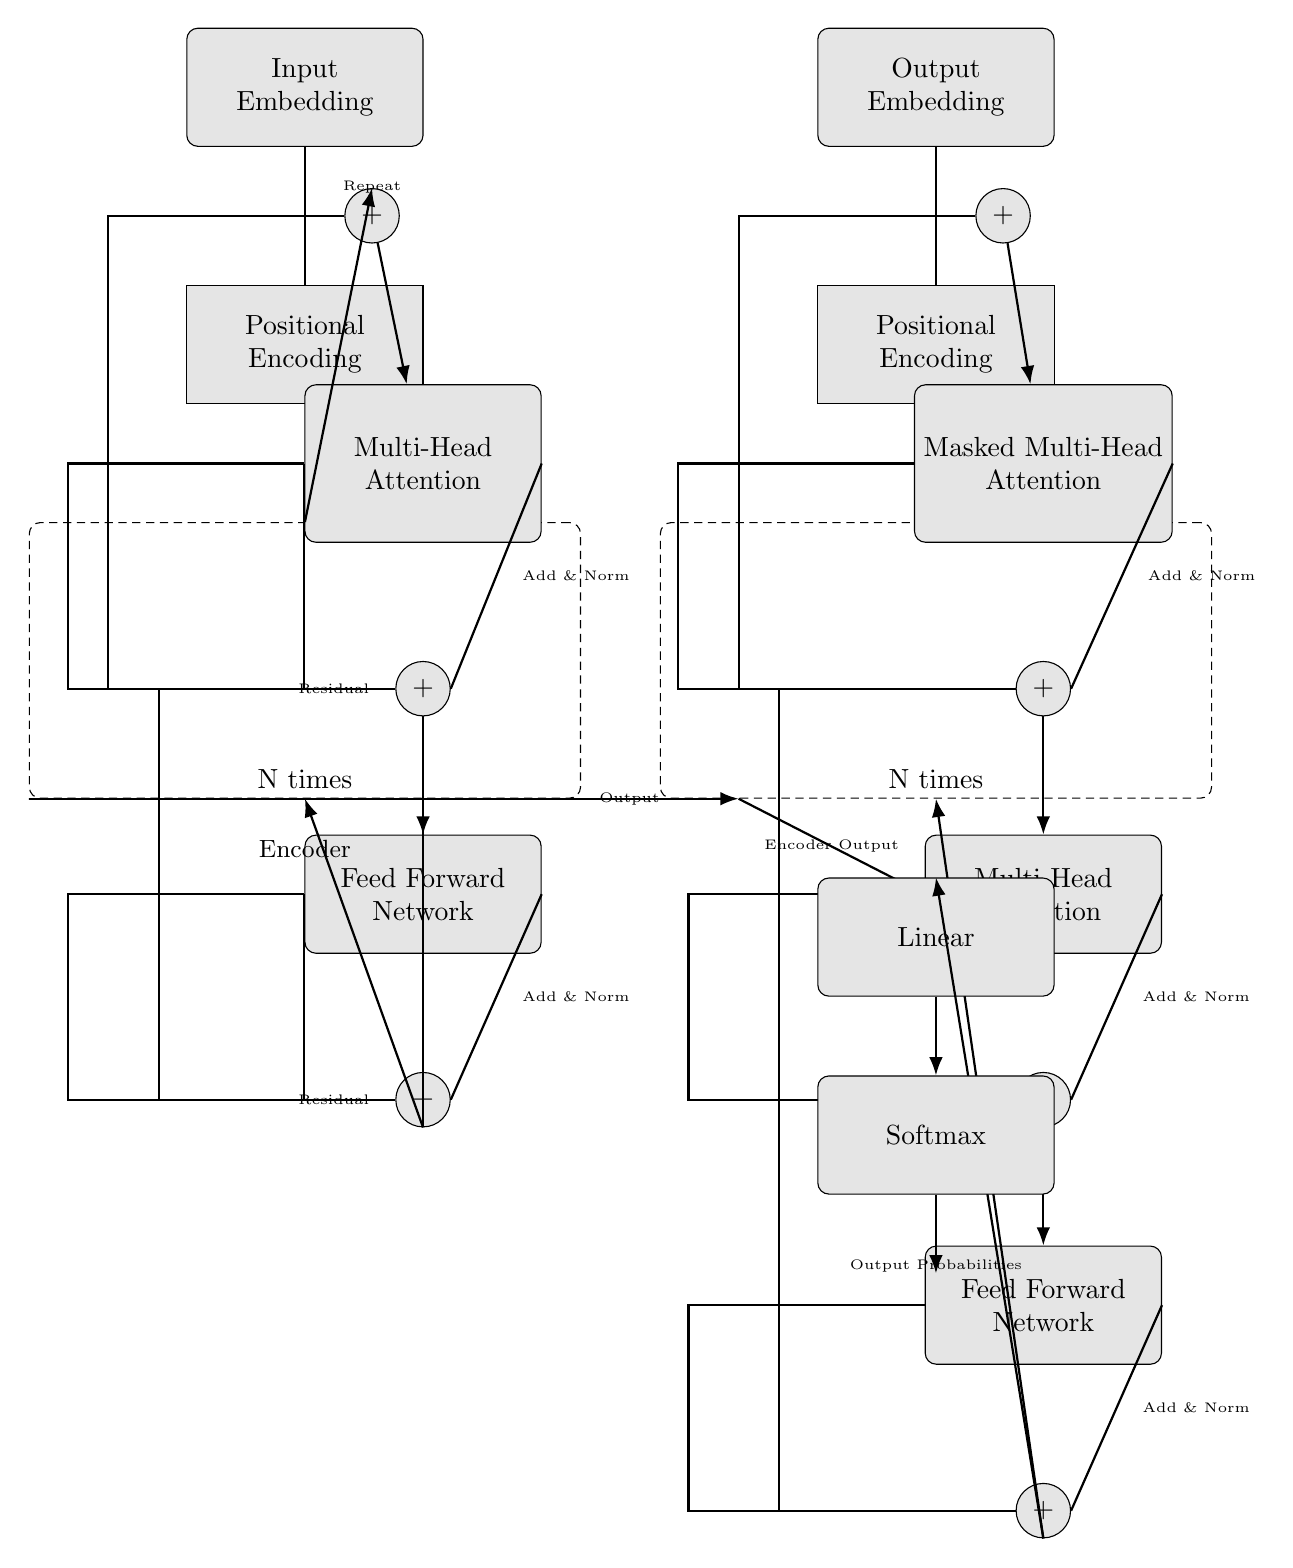
\begin{tikzpicture}[
    block/.style={
        draw, rectangle, rounded corners, minimum height=1.5cm,
        minimum width=3cm, align=center, fill=gray!20
    },
    process/.style={
        draw, rectangle, minimum height=1.5cm, minimum width=3cm,
        align=center, fill=gray!20
    },
    sum/.style={
        draw, circle, fill=gray!20, minimum size=6mm, align=center
    },
    repeat/.style={
        draw, rectangle, rounded corners, minimum height=3.5cm,
        minimum width=7cm, align=center, densely dashed
    },
    arrow/.style={-Latex,thick},
    line/.style={thick}
]

% Define positioning
\pgfmathsetmacro{\dx}{3.5}
\pgfmathsetmacro{\dy}{1.75}

% ============================== ENCODER ==============================
% ENCODER: Input processing
\node[block] (input_emb) {Input\\Embedding};
\node[process, below=\dy of input_emb] (pos_enc) {Positional\\Encoding};
\node[sum, right=0.5cm of $(input_emb.south)!0.5!(pos_enc.north)$] (sum_input) {+};

% ENCODER: Main block (Encoder layer)
\node[repeat, below=1.5cm of pos_enc, label={[yshift=0.5cm]below:N times}] (repeat_encoder) {};

\node[block, yshift=2.5cm, inner ysep=2pt, minimum height=2cm, left=0.5cm of repeat_encoder.east, anchor=east] (multihead_enc) {Multi-Head\\Attention};
\node[sum, below=1.5cm of multihead_enc] (sum_enc1) {+};
\node[block, below=1.5cm of sum_enc1] (ff_enc) {Feed Forward\\Network};
\node[sum, below=1.5cm of ff_enc] (sum_enc2) {+};

% ENCODER: Data flow
\draw[line] (input_emb.south) -- ($(input_emb.south)+(0,-\dy/2)$) coordinate (input_merge);
\draw[line] (pos_enc.north) -- ($(pos_enc.north)+(0,\dy/2)$);
\draw[line, bend left=90] (input_merge) to[out=180,in=180] (sum_input.west);
\draw[line] (input_merge) -- (sum_input.west);
\draw[arrow] (sum_input) -- (multihead_enc);
\draw[line] (multihead_enc.east) -- node[right,xshift=2mm,font=\tiny] {Add \& Norm} (sum_enc1.east);
\draw[arrow] (sum_enc1) -- (ff_enc);
\draw[line] (ff_enc.east) -- node[right,xshift=2mm,font=\tiny] {Add \& Norm} (sum_enc2.east);
\draw[arrow] (sum_enc2.south) -- (repeat_encoder.south);

% Encoder-specific residual connections
\draw[line] (sum_input) -- ($(sum_input.west)+(-3cm,0)$) |- (sum_enc1.west);
\draw[line] (multihead_enc) -- ($(multihead_enc.west)+(-3cm,0)$) |- (sum_enc1.west);
\draw[line] (sum_enc1) -- ($(sum_enc1.west)+(-3cm,0)$) |- (sum_enc2.west);
\draw[line] (ff_enc) -- ($(ff_enc.west)+(-3cm,0)$) |- (sum_enc2.west);


% Repeat block
\node[below=2mm of repeat_encoder.south,yshift=-2mm,font=\small] (enc_repeat_text) {Encoder};
\draw[arrow] (sum_enc2.south) |- (repeat_encoder.south west) -- (repeat_encoder.south east) node[right,xshift=1mm,font=\tiny](enc_out_text){Output} -- +(2cm,0) coordinate(enc_output);
\draw[arrow] (repeat_encoder.north) -- (sum_input.north) node[above,yshift=-2mm,font=\tiny] {Repeat};
\draw[line] (multihead_enc.west) -- (multihead_enc.west|-sum_enc1.west) -- (sum_enc1.west) node[left,xshift=-2mm,font=\tiny] {Residual};
\draw[line] (ff_enc.west) -- (ff_enc.west|-sum_enc2.west) -- (sum_enc2.west) node[left,xshift=-2mm,font=\tiny] {Residual};

% ============================== DECODER ==============================
% DECODER: Input processing
\node[block, right=5cm of input_emb] (output_emb) {Output\\Embedding};
\node[process, below=\dy of output_emb] (pos_enc_dec) {Positional\\Encoding};
\node[sum, right=0.5cm of $(output_emb.south)!0.5!(pos_enc_dec.north)$] (sum_output) {+};

% DECODER: Main block (Decoder layer)
\node[repeat, below=1.5cm of pos_enc_dec, label={[yshift=0.5cm]below:N times}] (repeat_decoder) {};

\node[block, yshift=2.5cm, inner ysep=2pt, minimum height=2cm, left=0.5cm of repeat_decoder.east, anchor=east] (masked_attn_dec) {Masked Multi-Head\\Attention};
\node[sum, below=1.5cm of masked_attn_dec] (sum_dec1) {+};
\node[block, below=1.5cm of sum_dec1] (multihead_dec) {Multi-Head\\Attention};
\node[sum, below=1.5cm of multihead_dec] (sum_dec2) {+};
\node[block, below=1.5cm of sum_dec2] (ff_dec) {Feed Forward\\Network};
\node[sum, below=1.5cm of ff_dec] (sum_dec3) {+};

% DECODER: Data flow
\draw[line] (output_emb.south) -- ($(output_emb.south)+(0,-\dy/2)$) coordinate (output_merge);
\draw[line] (pos_enc_dec.north) -- ($(pos_enc_dec.north)+(0,\dy/2)$);
\draw[line, bend left=90] (output_merge) to[out=180,in=180] (sum_output.west);
\draw[line] (output_merge) -- (sum_output.west);
\draw[arrow] (sum_output) -- (masked_attn_dec);
\draw[line] (masked_attn_dec.east) -- node[right,xshift=2mm,font=\tiny] {Add \& Norm} (sum_dec1.east);
\draw[arrow] (sum_dec1) -- (multihead_dec);
\draw[line] (multihead_dec.east) -- node[right,xshift=2mm,font=\tiny] {Add \& Norm} (sum_dec2.east);
\draw[arrow] (sum_dec2) -- (ff_dec);
\draw[line] (ff_dec.east) -- node[right,xshift=2mm,font=\tiny] {Add \& Norm} (sum_dec3.east);
\draw[arrow] (sum_dec3.south) -- (repeat_decoder.south);

% Decoder-specific residual connections
\draw[line] (sum_output) -- ($(sum_output.west)+(-3cm,0)$) |- (sum_dec1.west);
\draw[line] (masked_attn_dec) -- ($(masked_attn_dec.west)+(-3cm,0)$) |- (sum_dec1.west);
\draw[line] (sum_dec1) -- ($(sum_dec1.west)+(-3cm,0)$) |- (sum_dec2.west);
\draw[line] (multihead_dec) -- ($(multihead_dec.west)+(-3cm,0)$) |- (sum_dec2.west);
\draw[line] (sum_dec2) -- ($(sum_dec2.west)+(-3cm,0)$) |- (sum_dec3.west);
\draw[line] (ff_dec) -- ($(ff_dec.west)+(-3cm,0)$) |- (sum_dec3.west);


% Connect Encoder to Decoder
\draw[arrow] (enc_output) -- node[above,yshift=-2mm,font=\tiny] {Encoder Output} (multihead_dec.west);

% ============================== FINAL LAYER ==============================
\node[block, below=1cm of repeat_decoder, minimum width=3cm] (linear) {Linear};
\draw[arrow] (sum_dec3.south) -- (linear.north);

\node[block, below=1cm of linear, minimum width=3cm] (softmax) {Softmax};
\draw[arrow] (linear.south) -- (softmax.north);

\draw[arrow] (softmax.south) -- node[below,yshift=-2mm,font=\tiny] {Output Probabilities} +(0,-1cm);

\end{tikzpicture}

\end{document}

